\documentclass[letterpaper, 10 pt, conference]{ieeeconf}  
\IEEEoverridecommandlockouts\overrideIEEEmargins
\documentclass[10pt,a4paper]{report}
\usepackage[latin1]{inputenc}
\usepackage{amsmath}
\usepackage{amsfonts}
\usepackage{amssymb}
\usepackage{graphicx}
\usepackage{tikz}
\usepackage{tabularx}
\usetikzlibrary{matrix,calc}
\usepackage[margin=0.5in]{geometry}
\usepackage{tikz}
\usetikzlibrary{arrows,shapes.gates.logic.US,shapes.gates.logic.IEC,calc}
\begin{document}
\raggedright \begin{center} 
\includegraphics[scale=0.09]{iit_h.png} \end{center}

\vspace{10mm}
\raggedright\textbf\ \hspace{1mm} \  Assignment 1\hspace{6cm}
 \  Name:\hspace{1mm}Dulla Srinivas\hspace{5cm} \hspace{4cm} 
roll no :\hspace{1mm} FWC22041\vspace{2cm}
\raggedright \\PROBLEM STATEMENT:\vspace{2mm}
\raggedright \\ state and Prove Commutative Law
\raggedright \\The definition of commutative law states that when we add or multiply two numbers then the resultant value remains the same, even if we change the position of the two numbers. Or we can say, the order in which we add or multiply any two real numbers does not change the result.
\vspace{1cm}
\\ sollution: A+B = B+A
 \\ \hspace{15mm} A.B = B.A
\vspace{5mm}
\\\textbf{\underline{Components:}}\vspace{2mm}
\begin{table}[ht]
\centering % used for centering table
\begin{tabular}{c c c} % centered columns (4 columns)
\hline\hline %inserts double horizontal lines
S.No & Component & Number \\ [0.5ex] % inserts table 
\hline
1 & Arduino & 1 \\
2 & Bread Board & 1 \\
3 & Jumer Wires(M-M) & 3\\
\hline
\end{tabular}
\end{table}

\vspace{5mm}
\\ \raggedright \textbf{\underline{Procedure:}}\vspace{2mm}
\\ \raggedright 1) First make the 8 digital output pins of arduino to breadboard 
\\ 2) connect GND to breadboard
\\ 3)with help of resistor connect led to arduino board
\\ 4)Write the given logic in code and upload in to the arduino.
 

\begin{figure}

    \centering
    

    \caption{Caption}
    \label{fig:my_label}
\end{figure}
\vspace{5mm}


\vspace{7mm}
\\ \raggedright \textbf{\underline{Truthtable: A+B=B+A}}\vspace{2mm}
\begin{table}[ht]
\centering % used for centering table
\begin{tabular}{c c c c c} % centered columns (4 columns)
\hline\hline %inserts double horizontal lines
 \textbf{A} & \textbf{B} & \textbf{A+B} &\textbf{B+A}\\ [0.5ex] % inserts table 
\hline
      0 & 0 & 0 & 0\\
      0 & 1 & 1 & 1\\
      1 & 0 & 1 & 1\\
      1 & 1 & 1 & 1\\
\hline
\end{tabular}
\end{table}
\\ \raggedright \textbf{\underline{Truthtable: A.B=B.A}}\vspace{2mm}
\begin{table}[ht]
\centering % used for centering table
\begin{tabular}{c c c c c} % centered columns (4 columns)
\hline\hline %inserts double horizontal lines
  \textbf{A} & \textbf{B} & \textbf{AB} &\textbf{BA}\\ [0.5ex] % inserts table 
\hline
      0 & 0 & 0 & 0\\
      0 & 1 & 0 & 0\\
      1 & 0 & 0 & 0\\
      1 & 1 & 1 & 1\\
\hline
\end{tabular}
\end{table}
\raggedright \textbf{\underline{Code:}}\vspace{7mm}
\\ you may  refer these code in github  \hspace{1mm}
link    :https://github.com/Dsrinivas-sudo?tab=repositories

\vspace{2cm}
\\.include "/home/fwc assembly/m328Pdef.inc"
\\ldi r16, 0b00000001 ;  
\\out DDRB,r16; declare 8th pin as a output 



\\ldi r16,0b00000000; perform or operation by compating two 
\\ldi r17,0b00000001;
\\mov r18,r16;
\\and r16,r17;
\\and r17,r18;

\\cp r16,r17;  comapre r16 with r17
\\breq lbl; 

\\lbl:
\\eor r16,r17; performing xor operation
\\COM r16;
\\out PORTB,r16;
\\start: rjmp start
\\
\vspace{1cm}
\raggedright \textbf{\underline{Output:}}\vspace{7mm} 
\raggedright \begin{center} 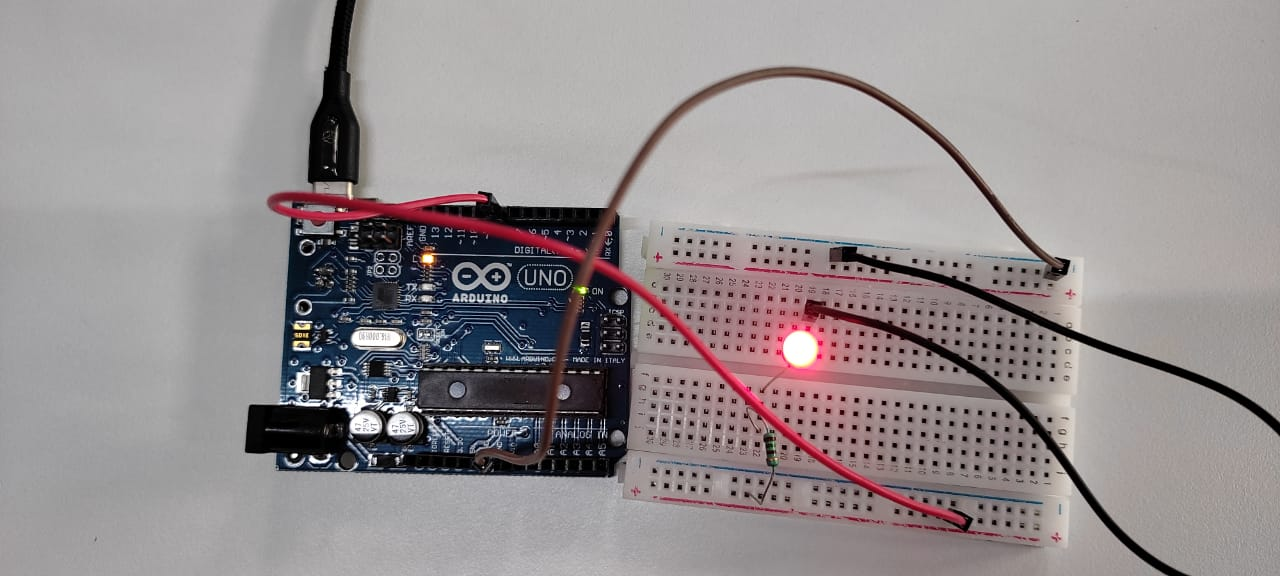
\includegraphics[scale=0.09]{out.jpg} \end{center}


\raggedright \textbf{\underline{Conclusion:}}\vspace{7mm}
\\ Hence have implemented the commulative law of boolean algebra in arduino and verified the outputs.
\\ we implement code in assembly level language and verified the outputs
\end{document}